\documentclass[a4paper]{article}
\usepackage[utf8]{inputenc}
\usepackage[spanish, es-tabla, es-noshorthands]{babel}
\usepackage[table,xcdraw]{xcolor}
\usepackage[a4paper, footnotesep = 1cm, width=18cm, left=2cm, top=2.5cm, height=25cm, textwidth=18cm, textheight=25cm]{geometry}
%\geometry{showframe}

\usepackage{tikz}
\usepackage{amsmath}
\usepackage{amsfonts}
\usepackage{amssymb}
\usepackage{float}
\usepackage{graphicx}
\usepackage{caption}
\usepackage{subcaption}
\usepackage{multicol}
\usepackage{multirow}
\setlength{\doublerulesep}{\arrayrulewidth}
\usepackage{booktabs}

\usepackage{hyperref}
\hypersetup{
    colorlinks=true,
    linkcolor=blue,
    filecolor=magenta,      
    urlcolor=blue,
    citecolor=blue,    
}
\newcommand\underrel[2]{\mathrel{\mathop{#2}\limits_{#1}}}
\newcommand{\quotes}[1]{``#1''}
\usepackage{array}
\newcolumntype{C}[1]{>{\centering\let\newline\\\arraybackslash\hspace{0pt}}m{#1}}
\usepackage[american]{circuitikz}
\usetikzlibrary{calc}
\usepackage{fancyhdr}
\usepackage{units} 

\graphicspath{{../Ejercicio-1/}{../Ejercicio-2/}{../Ejercicio-3/}}

\pagestyle{fancy}
\fancyhf{}
\lhead{22.13 Electrónica III}
\rhead{Mechoulam, Lambertucci, Martorell, Londero}
\rfoot{\center \thepage}
\usepackage{multirow}
\begin{document}

\section{Ejercicio 2}
\subsection{Introdución}
En esta sección se procederá a realizar una máquina de estados capaz de detectar la secuencia de bits 1-1-0-1.

\subsection{Implementación} 
Para poder realizar esta detector de secuencias se consideró que el último bit de la secuencia puede ser el primero de una nueva, por ejemplo, si viene una cadena de bits de la siguiente forma 1-1-0-1-1-0-1 la máquina de estados detectará dos secuencias correctas de bits. A su vez se consideró que si un caracter es incorrecto la máquina de estado vuelve a su estado base inicial y se vuelve a comenzar. Se realizo el siguiente diagrama de estados utilizando una máquina de Mealy:
\begin{figure}[H]
\centering

\includegraphics{ImagenesEjercicio2/pend.jpg}
\caption{Diagrama de la máquina de Mealy utilizada para detectar la secuencia de bits}
\end{figure}


Otorgandole a los estados la siguiente numeración: $A=00$, $B=01$, $C=10$, $D=11$, se obtiene la siguiente tabla:

\begin{table}[H]
\centering
\begin{tabular}{ccccc}
\multirow{2}{*}{Estado actual} & \multicolumn{2}{c}{Próximo estado} & \multicolumn{2}{c}{Salida} \\
 & w=0 & w=1 & w=0 & w=1 \\
$y_2y_1$ & $Y_2Y_1$ & $Y_2Y_1$ & $Z$ & $Z$ \\
A & A(00) & B(01) & 0 & 0 \\
B & A(00) & C(10) & 0 & 0 \\
C & D(11) & A(00) & 0 & 0 \\
D & A(00) & B(01) & 0 & 1
\end{tabular}
\end{table}

A partir de esta tabla se realizaron los respectivos mapas de karnaugh para las salidas $Y_1$, $Y_2$, se pudo observar que tanto para maxtérminos como para mintérminos el número de operaciones lógicas a realizar eran las mismas, por lo tanto se optó por utilizar los mintérminos y se obtuvo los siguientes mapas:

\begin{figure}[H]
\centering
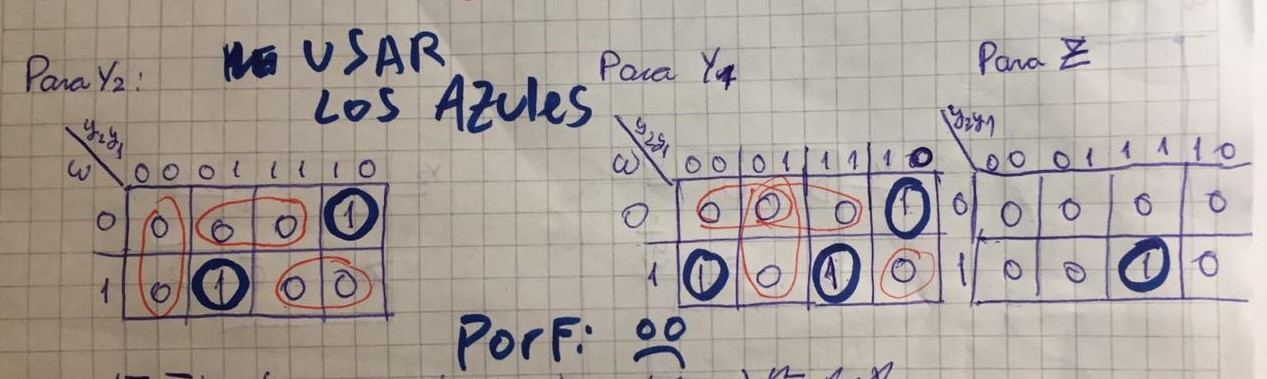
\includegraphics{ImagenesEjercicio2/mapitas.jpg}
\caption{Mapas de karnaugh primero del primer Flip-Flop, luego del segundo y por último la salida deseada}
\end{figure}
Con los que se obtienen las siguientes funciones:
$Y_1=(w\bar{y_2}\bar{y_1})+(wy_1y_2)+(\bar{w}y_2\bar{y_1})$
$Y_2=(w\bar{y_2}y_1)+(\bar{w}y_2\bar{y_1})$
$Z=wy_2y_1$
Utilizando 2 flip-flops tipo D para representar las 4 combinaciones posibles para obtener todos los posibles estados, considerando que los proximos estados se pueden representar como la entrada de dichos flip-flops y la salida de estos como el estado actual, se presenta el siguiente circuito:
\begin{figure}[H]
\centering
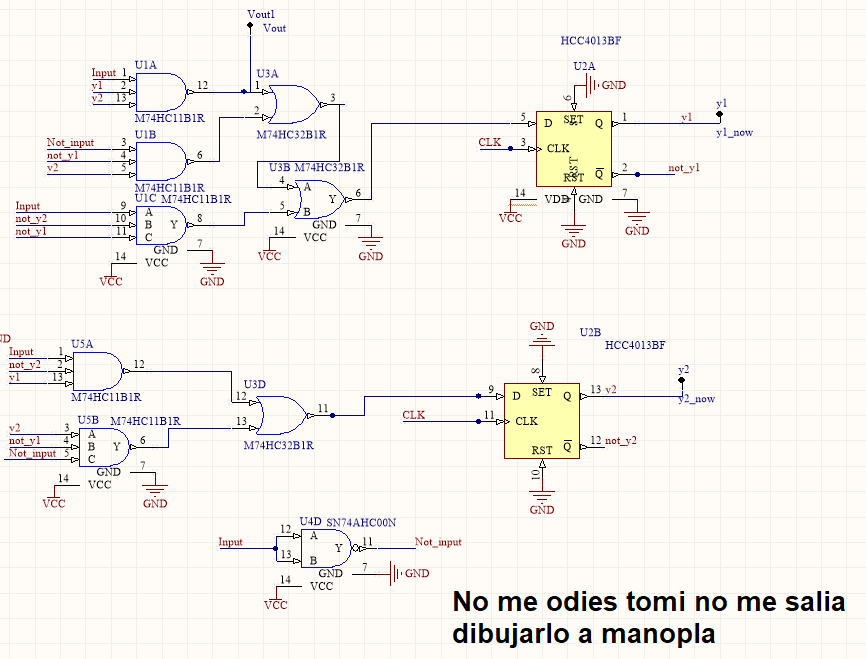
\includegraphics{ImagenesEjercicio2/circuito.jpg}
\caption{Circuito a implimitar que cumple con la maquina de estados deseada}
\end{figure}
\end{document}

Consecuentemente se procedio a realizar la simulación en verilog de dicho circuito con la que se obtuvo los siguientes resultados:

\begin{figure}[H]
\centering
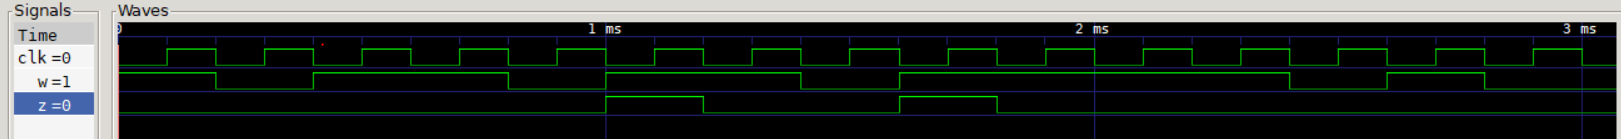
\includegraphics{ImagenesEjercicio2/simulacion.png}
\caption{Simulaciones en GTKwave, donde w simboliza la entrada, z la salida y clk el clock del circuito}
\end{figure}
\end{document}

Como era de esperarse dicho circuito emula satisfactoriamente la máquina de estados planteada, por lo que se puede detectar correctamente la secuencia de bits deseados cuando esta se presenta. Ulteriormente de las simulaciones se procedio a diseñar dicho circuito en PCB con el cual se obtuvieron los mismos resultados por lo que se corroboró el correcto funcionamiento de la máquina de estados implementada, como se puede presenciar en las siguientes figuras.

\begin{figure}[H]
\centering
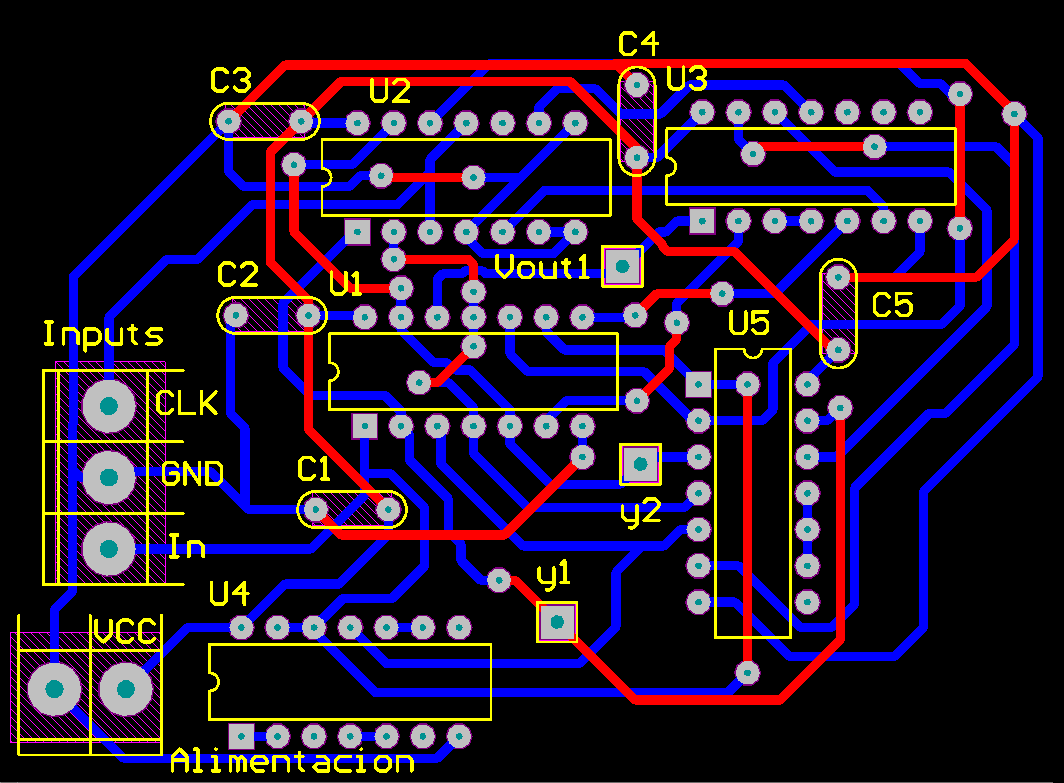
\includegraphics{ImagenesEjercicio2/pcb.png}
\caption{Implementación en PCB del circuito implementado }
\end{figure}
\end{document}

\begin{figure}[H]
\centering

\includegraphics{ImagenesEjercicio2/pend.jpg}
\caption{Detección de la secuencia deseada vista en el osciloscopio }
\end{figure}
\end{document}

